\section{Examen 2.- Administración de fallas usando series de datos no lineales mediante Holt Winters}
\subsection{Evidencia 1}
Nos fue proporcionada una base de datos round robin (predict.rrd), el cual contenía las mediciones hechas para el objeto de la mib ``ifInOctets''. Esto con la finalidad de que nosotros determinaramos si los valores de alpha, beta y gamma eran los adecuado para realizar el monitoreo o podían mejorar.\\Para esto, lo primero que realizamos, fue graficar el archivo rrd con la intención de obtener información de esta gráfica. La gráfica obtenida puede observarse en la figura \ref{img:1-1}.
\begin{figure}[H]
  \centering
    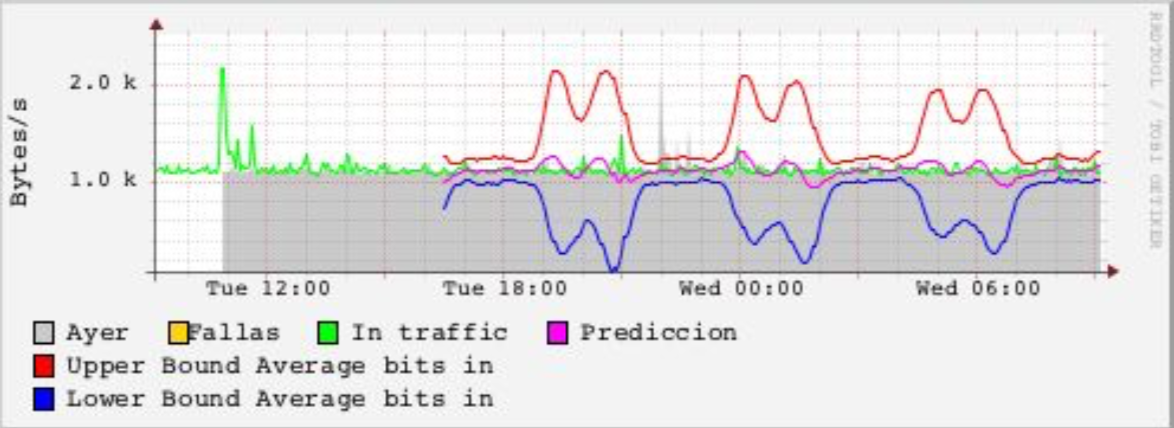
\includegraphics[scale=.75]{imagenes/segundo/1.png}
    \caption{Gráfica obtenida del archivo rrd}
    \label{img:1-1}
\end{figure}
Como se puede observar, la gráfica obtenida muestra el tráfico de entrada de color verde, los límites superior e inferior de color rojo y azul respectivamente, y la predicción de holt-winters de color rojo. Así como también el histórico de datos leidos de color gris.\\Posterior al análisis de la gráfica, se determino que los valores de alpha, beta y gamma se mantuvieran como los mismos, ya que la predicción era bastante cercana a los valores reales.\\Cabe señalar, que los valores de alpha, beta y gamma eran conocidos, gracias al ``dump'' hecho al archivo rdd, el cual genera un archivo xml desde el cual se pueden consultar estos valores.\\En caso de que hubiera sido necesario modificar el valor de alguno de estos valores, se puede usar la función ``tune'', con el cual se pueden modificar estos parámetros. Esto se puede observar en la figura \ref{img:1-2}.
\begin{figure}[H]
  \centering
    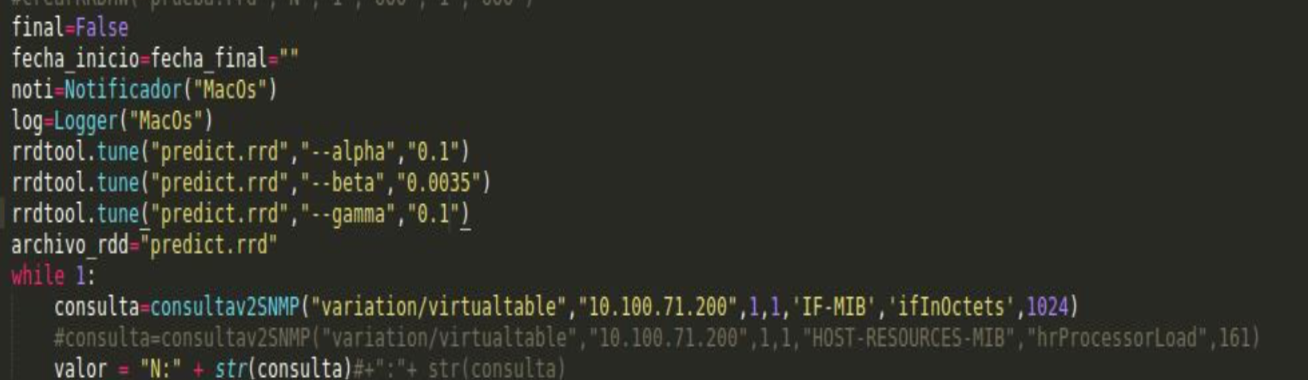
\includegraphics[scale=.75]{imagenes/segundo/2.png}
    \caption{Uso de la función tune}
    \label{img:1-2}
\end{figure}

\subsection{Evidencia 2}
Para la siguiente parte del examen, se nos pidió detectar una falla (comportamiento anormal que sobrepasas uno de los límites) y mostrar la gráfica correspondiente donde se observe como se coloea de color rojo el area donde se muestra la falla detectada.\\ En la figura \ref{img:1-3}
\begin{figure}[H]
  \centering
    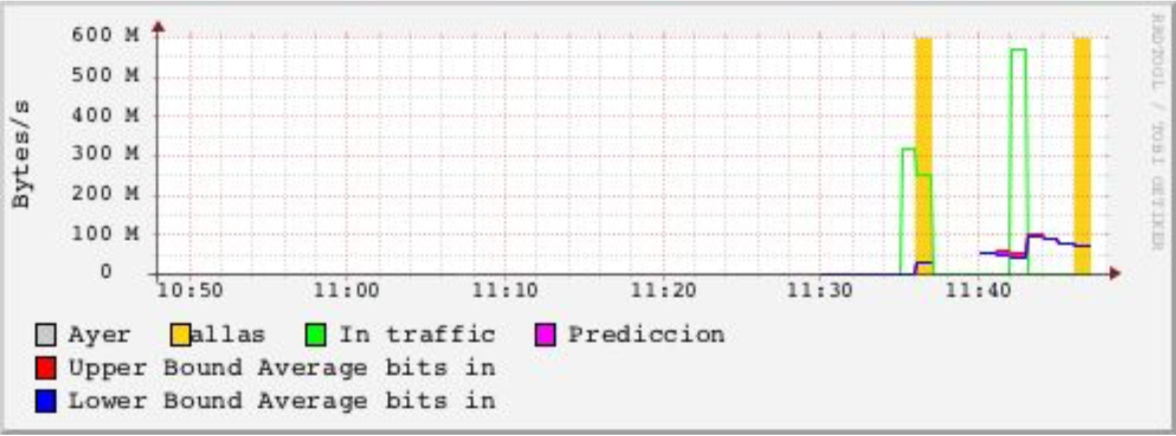
\includegraphics[scale=.75]{imagenes/segundo/3.png}
    \caption{Gráfica que muestra como se detecta un fallo}
    \label{img:1-3}
\end{figure}
Además, se nos solicito, que se mostrará el histórico de las mediciones hechas en un tiempo anterior al actual, esto puede observarse en la figura \ref{img:1-4} con el área marcada de color gris.
\begin{figure}[H]
  \centering
    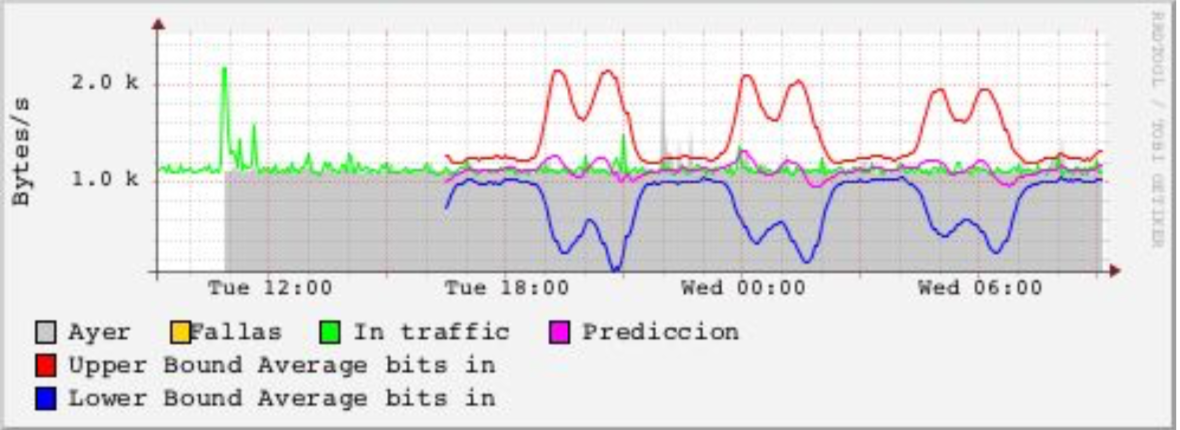
\includegraphics[scale=.75]{imagenes/segundo/4.png}
    \caption{Gráfica que muestra el histórico coloreado.}
    \label{img:1-4}
\end{figure}
\subsection{Evidencia 3}
Finalmente, fue necesario enviar una notificación al administrador, vía correo electrónico, cuando se presentarña alguna falla, estas notificaciones tenían que enviarse, al iniciar una falla y al culminar, en estas notificaciones, se incluye la información del agente donde se presentó el problema, la fecha y hora, y además una imagen que muestra la gráfica que es generada en tiempo real del rendimiento del objeto mib.\\En la figura \ref{img:1-5} se muestra uno de los correos que fue enviado.
\begin{figure}[H]
  \centering
    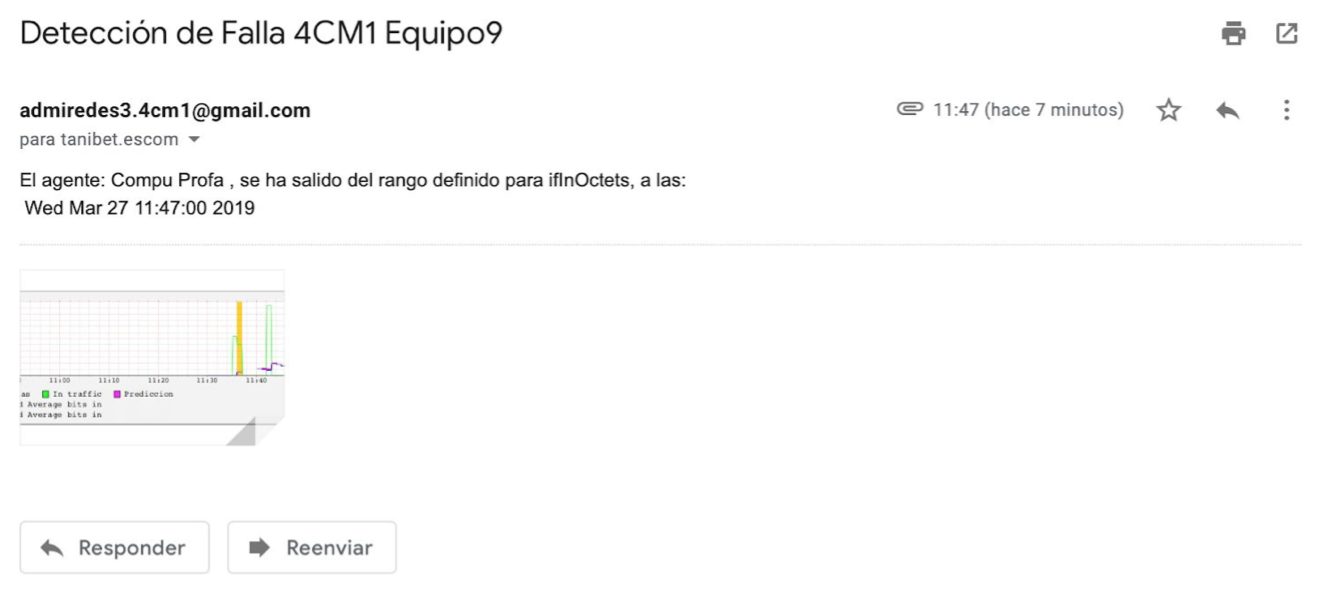
\includegraphics[scale=.75]{imagenes/segundo/5.png}
    \caption{Notificación enviada al detectarse una falla.}
    \label{img:1-5}
\end{figure}
